%\begin{textblock}{9}(2.5,-3)
%\begin{flushright}
%\setlength{\baselineskip}{15pt}
%\textblockrulecolour{white}
%~
%
%``Mi investigación en la física ha consistido en simplemente examinar cantidades matemáticas de un tipo que los físicos usan y tratar de relacionarlas de una manera interesante.''\\[.5cm]
%\textit{Paul A. M. Dirac.}
%\end{flushright}
%\end{textblock}

En este capítulo se presenta la simulación, tratamiento y análisis de la señal de decaimiento del higgs a dos di-muones fundamentado en la teoría \textbf{Dark-}\SUSY~ (ver Fig. \ref{fig:sketch_darksector}b), bajo diferentes condiciones de los detectores \CMS. 


Este proyecto se organizó en cuatro etapas en como se observa en el diagrama de la Fig. \ref{procesos_darksusy}. Primeramente, se genera la simulación de los decaimiento bajo diferentes condiciones iniciales, buscando que sea suficientemente flexible a distintas condiciones de trabajo sin perder la eficiencia en el proceso de implementación computacional.
\begin{figure}[!b]
\centering
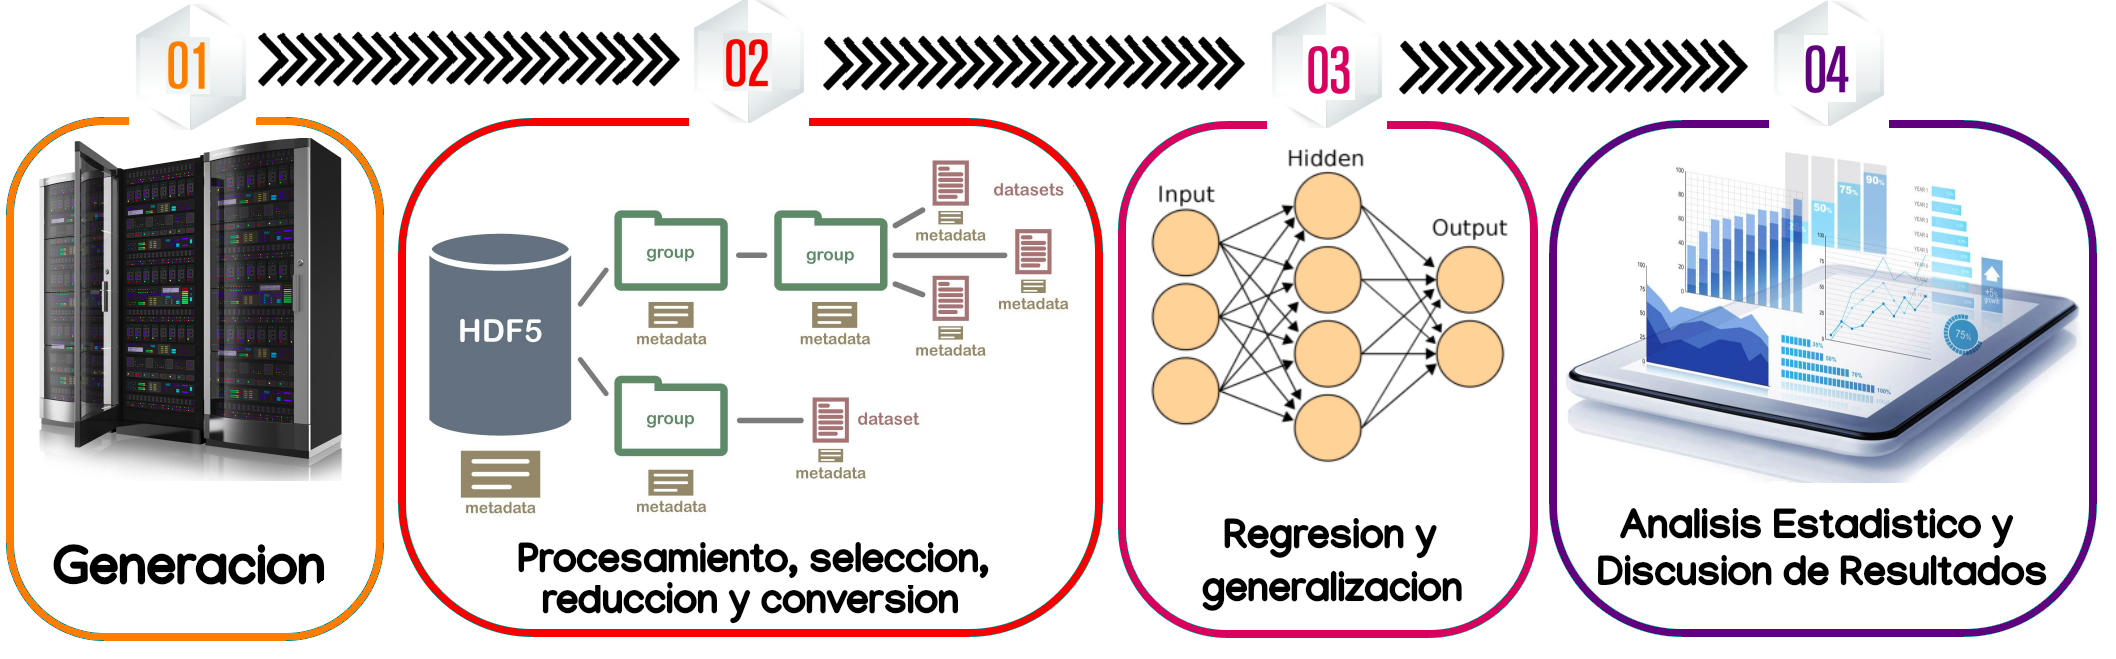
\includegraphics[width=1\textwidth]{Simulacion/imagenes/procesos_darksusy.png}
\caption{Secuencia lógica del análisis del proyecto.}
\label{procesos_darksusy}
\end{figure}
La información pertinente al estudio es extraída de la simulación y almacenada en formato \textbf{HDF}. Posteriormente se ajustan modelos de regresión para generalizar la información haciendo uso de herramientas de regresión y tratamiento de datos con redes neuronales. Finalmente, se hace un estudio estadístico y análisis de los resultados.

%La información recopilada debe ser debidamente procesada, dada las limitantes tecnológicas a las que se tiene acceso, de tal forma, que permita la reconstrucción de resultados en condiciones cercanas a las ya conocidas, existen en el ámbito científico varios métodos para abordar esta problemática uno de los más sencillo es el hacer uso de herramientas de regresión y tratamiento de datos con redes neuronales, este forma parte del tercer grupo de herramientas desarrolladas. Finalmente se procederá al desarrollo de las herramientas para realizar el análisis estadístico característico de la física del proceso al que se le está estudiando, su interpretación y discusión es la intencionalidad final del trabajo. 


%El proceso de simulación genera mucha no pertinente a la investigación actual

%Los resultados anteriormente referidos estarán en un formato típicamente inadecuado para realizar un estudio en particular, esto consecuencia del gran tamaño de los archivos obtenidos, y la alta dispersión de la información relevante a la investigación, de aquí que la reconstrucción de la información de los eventos requeridos en archivos de formato de datos jerárquico $\mathbf{*.h5}$ permitiendo una mayor rapidez en el acceso.


La información recopilada debe ser debidamente procesada, dada las limitantes tecnológicas a las que se tiene acceso, de tal forma, que permita la reconstrucción de resultados en condiciones cercanas a las ya conocidas, existen en el ámbito científico varios métodos para abordar esta problemática uno de los más sencillo es el hacer uso de herramientas de regresión y tratamiento de datos con redes neuronales, este forma parte del tercer grupo de herramientas desarrolladas. Finalmente se procederá al desarrollo de las herramientas para realizar el análisis estadístico característico de la física del proceso al que se le está estudiando, su interpretación y discusión es la intencionalidad final del trabajo. 

% siendo este un estándar de uso general, independiente de la máquina para almacenar datos científicos en archivos, desarrollado por el centro nacional para aplicaciones de Supercomputación (NCSA). HDF5 es utilizado por una amplia gama de campos de ingeniería y científicos que quieren una forma estándar de almacenar datos para que puedan compartirse. Para obtener más información sobre el formato de archivo HDF5, lea la documentación de HDF5 disponible en el sitio web de HDF (https://www.hdfgroup.org). 



%estos son programados en \textbf{Python} y \textbf{C++}, la explicación de estas herramientas darán las bases para profundizar en los resultados obtenidos y su respectiva discusión.

%necesarios para cumplir con el objetivo de esta investigación, recreando y estudiando 